%% -*- coding:utf-8 -*-

\chapter{Empty elements}
\label{Abschnitt-Diskussion-leere-Elemente}
\label{chap-empty}

This chapter deals with empty elements, I first discuss the general attitude of various research
traditions towards empty elements and then show how they can be eliminated from grammars
(Section~\ref{Abschnitt-Eleminierung-leerer-Elemente}). Section~\ref{Abschnitt-leere-Elemente-Semantik} discusses empty elements that
have been suggested in order to facilitate semantic
interpretation. Section~\ref{Abschnitt-Evidenz-leere-Elemente} discusses possible motivation for
empty elements with a special focus on cross"=linguistic comparison and the final Section~\ref{Abschnitt-leere-Elemente-LRs-Transformations} shows
that certain accounts with transformations, lexical rules, and empty elements can be translated into each other.

\section{Views on empty elements}

One\is{empty element|(} point that is particularly controversial among proponents of the theories discussed in this book is the question of whether
one should assume empty elements or not.\todostefan{Add arguments from wanna contraction} The discussion of empty elements is quite old: there was already some investigation in 1961 with reference
to phrase structure grammars\is{phrase structure grammar} \citep*{BHPS61a}.
The discussion of the status of empty elements has carried on ever since (see
\citealp*{Loebner86a,Wunderlich87d,Wunderlich89,Stechow89,Haider97a,Sag2000a,BMS2001a,LH2006a,Mueller2004e,AS2015a}, for example). 
There are sometimes empirical differences between analyses that assume empty elements and those that
do not \citep{AS2015a}, but often this is not the case. Since empty elements often feature prominently in the argumentation for or against particular theories, I will discuss
how they have been used in somewhat more detail here.

In \gbt, empty elements were assumed for traces of movement (verb movement and fronting of phrases) as well as for deleted elements in 
elliptical\is{ellipsis} constructions. Starting with the analysis of \citet{Larson88a}, more and more empty heads have been introduced to ensure uniformity\is{uniformity} of structures and 
certain semantic interpretations (binding\is{Binding Theory}
and scope\is{scope}, see Section~\ref{sec-little-v} on \littlev). Other examples of an empty element that was introduced in order to maintain particular generalizations are the empty expletives\is{pronoun!expletive}
of \citet[\page 734]{Coopmans-89a-u} and \citet[Chapter~1]{Postal2004a-u}. These fill the subject
position in inversion\is{inversion} structures in English\il{English}, where the position preceding
the verb is occupied by a PP and not by an overt subject NP. Similarly, \citet[\page
  1311]{Grewendorf93} assumes that the subject position in impersonal
passives\is{passive!impersonal} and passives without subject movement is in fact occupied by an
empty expletive. Also, see
\citew[\page 91]{Newmeyer2005a} and \citet[\page 180]{Lohnstein2014a} for this assumption with regard to the passive
in German. \citet[Section~II.3.3.3]{Sternefeld2006a-u} assumes that there is an empty expletive subject in impersonal passives and subjectless sentences such as
(\mex{1}).
\eal
\ex 
\gll Mir graut.\\
	 me.\dat{} scares\\
\glt `I am scared.'
\ex 
\gll Mich dürstet.\\
	 me.\acc{} is.thirsty\\
\glt `I am thirsty.'
\zl

\noindent
On page~\pageref{Beispiel-leeres-Element-intransitive-Verben}, we discussed Stabler's proposal for the analysis of sentences with intransitive
verbs. Since, following  \citet[\page 146]{Chomsky2008a}, the element that first merges with a head is the complement, intransitive verbs pose a problem for the
theory. This problem is solved by Stabler by assuming that intransitive verbs are combined with an empty object \citep[\page 61,
124]{Veenstra98a}. Since these silent elements do not contribute to the meaning of an expression, we are also dealing with empty expletive pronouns.

\addlines
In other theories, there are researchers that reject empty elements as well as those who assume them.
In Categorial Grammar\indexcg, Steedman suggests an analysis of nonlocal dependencies that does
without empty elements (see Section~\ref{sce-nld-cg}), but as \citet{Pollard88a} has shown,
Steedman's analysis requires various kinds of type raising\is{type raising}
for NPs or a correspondingly high number of complex lexical items for relative pronouns\is{pronoun!relative} (see Section~\ref{Abschnitt-CG-UDC}). On the other hand,
\citet{Koenig99a-u} uses\todostefan{andere Quellen?}
traces. In GPSG\indexgpsg, there is the trace"=less analysis of extraction\is{extraction} by \citet[\page 76--77]{Uszkoreit87a} that we discussed in 
Section~\ref{Abschnitt-GPSG-Fernabhaengigkeiten}, but there is also the analysis of \citet*[\page 143]{GKPS85a} that uses traces. In LFG\indexlfg, there are both analyses with
traces \citep[\page 67]{Bresnan2001a} and those without (see \citew{KZ89a,DKK2001a-u} and Section~\ref{Abschnitt-Verbstellung-LFG} and Section~\ref{Abschnitt-NLA-LFG}). 
Many of the phrasal analyses in HPSG\indexhpsg are born out of the wish to avoid empty elements (see Section~\ref{Abschnitt-Phrasale-Konstruktionen}). 
An example for this is the relative clause analysis by \citet{Sag97a} that replaces the empty
relativizer in \citew{ps2} with a corresponding phrasal rule. On the other hand we have
\citew{Bender2000a} and \citew*[\page 464]{SWB2003a}, who assume a silent copula\is{copula}. Another attempt to eliminate empty elements from HPSG was to handle
long"=distance dependencies not by traces but rather in the lexicon \citep*{BMS2001a}. As \citet{LH2006a} could show, however, theories of extraction that
introduce long"=distance dependencies lexically have problems with the semantic interpretation of coordinate structures. For a suggestion of how to solve these problems,
see \citew{Chaves2009a}. There are many TAG analyses\indextag without silent elements in the lexicon (see Section~\ref{TAG-Fernabh} and \citew{Kroch87a}, for example),
however there are variants of TAG such as that of \citet[\page 194]{Kallmeyer2005a-u}, where a trace is assumed for the reordering of constituents in sentences with
a verbal complex. \citet[\page 10--11]{Rambow94a} assumes an empty head in every verb
phrase (see Section~\ref{sec-vtag} on V"=TAG\is{Tree Adjoining Grammar (TAG)!Vector (V-TAG)}).\footnote{
  Note that empty elements in TAG are slightly different from empty elements in other theories. In
  TAG the empty elements are usually part of elementary trees, that is, they are not lexical items that are
  combined with other material.
}
In Dependency Grammar, \mel (\citeyear[\page 303]{Melcuk88a-u}; \citeyear[\page 219]{Melcuk2003a-u}),
%\todostefan{S: It is possible to introduce empty nodes in a DT if you want. It has been done for
%  gapping by Tesnière or for agreement by Melcuk (1988:303)}
%\todostefan{O: Starosta 1988:253, Eroms 2000:472, Melcuk 2003:219, Hudson (2007:172-182, 2010)}
\citet[\page 253]{Starosta88a-u}, \citet[\page 471--472]{Eroms2000a}, Hudson (\citeyear[Section~3.7]{Hudson2007a-u}; \citeyear[\page 166]{Hudson2010a-u}) and
\citet{Engel2014a} assume empty elements for determiners, nouns, ellipsis, imperatives, controlled infinitives, and for coordinate
structures, but \citet[\page 73]{GO2009a} reject empty elements (with the exception of ellipsis, \citealp{Osborne2016a-u}).

No empty elements are assumed in Construction Grammar\indexcxg\label{Seite-leere-Elemente-CxG} (\citealp[\page 49--50]{MR2001a}; \citealp[\page
219]{Goldberg2003b}; \citealp[\page 10]{Goldberg2006a}), the related Simpler Syntax \citep{CJ2005a} as well as in Cognitive Grammar\is{Cognitive Grammar}.\footnote{
  However, \citet[\page 51]{Fillmore88a} did not rule them out.
} 
The argumentation against empty elements runs along the following lines:
\begin{enumerate}
\item There is no evidence for invisible objects.
\item There is no innate linguistic knowledge.
\item Therefore, knowledge about empty elements cannot be learned, which is why they cannot be assumed
as part of our grammar.
\end{enumerate}
This begs the question of whether all the premises on which the conclusion is based actually hold. If we consider an elliptical
construction such as (\mex{1}), then it is clear that a noun has been omitted:
\ea
\gll Ich nehme den roten Ball und du den blauen.\\
	 I take the.\acc{} red.\acc{} ball and you the.\acc{} blue.\acc{}\\
\glt `I'll take the red ball and you take the blue one.'
\z
Despite there being no noun in \emph{den blauen} `the blue', this group of words behaves both syntactically and semantically just like a noun
phrase. (\mex{0}) is of course not necessarily evidence for there being empty elements, because one could simply say that \emph{den blauen}
is a noun phrase consisting only of an article and an adjective \citep{Wunderlich87d}. 

Similar to the fact that it is understood that a noun is missing in (\mex{0}), speakers of English know that something is missing after
\emph{like}: 
\ea
Bagels, I like.
\z
Every theory of grammar has to somehow account for these facts. It must be represented in some way that \emph{like} in (\mex{0}) behaves
just like a verb phrase that is missing something. One possibility is to use traces. \citet*[\page 153, Lemma~4.1]{BHPS61a} 
have shown that it is possible to turn phrase structure grammars with empty elements into those without any.
In many cases, the same techniques can be applied to the theories presented here and we will therefore discuss the point in more detail
in the following section.

\section{Eliminating empty elements from grammars}
\label{Abschnitt-Eleminierung-leerer-Elemente}

It is possible to turn a grammar with empty elements (also called \emph{epsilon}\is{epsilon}) into a
grammar without these by removing all categories that can be rewritten by an epsilon in every rule
that uses such categories and then add the respective rules without the empty elements to the grammar. The following example has an epsilon rule for np. One therefore has to
replace all rules containing the symbol np with new rules without this np symbol. (\mex{2}) shows
the result of this conversion of the grammar in (\mex{1}):

\ea
\label{ex-grammar-eps-head}
\begin{tabular}[t]{@{}l@{~$\to$~}l@{}}
\baro{v}   & \mbox{np}, v\\
\baro{v}   & \mbox{np}, pp, v\\
np & $\epsilon$\\
\end{tabular}
\z

\ea
\label{ex-grammar-head}
\begin{tabular}[t]{@{}l@{~$\to$~}l@{}}
\baro{v}   & \mbox{np}, v\\
\baro{v}   & v\\
\baro{v}   & \mbox{np}, pp, v\\
\baro{v}   & \mbox{pp}, v\\
\end{tabular}
\z
This can also lead to cases where all elements on the right"=hand side of a rule are removed. Thus,
what one has done is actually create a new empty category and then one has to apply the respective
replacement processes again. We will see an example of this in a moment. Looking at the pair of
grammars in (\mex{-1})--(\mex{0}), it is clear that the number of rules has increased in (\mex{0})
compared to (\mex{-1}) despite the grammars licensing the same sequences of symbols. The fact that
an NP argument can be omitted is not expressed directly in (\mex{0}) but instead is implicitly contained in two rules. 

If one applies this procedure to the HPSG\indexhpsg grammar in Chapter~\ref{Kapitel-HPSG}, then the
trace does not have a specific category such as NP. The trace simply has to be compatible with a
non"=head daughter. As the examples in (\mex{1}) show, adjuncts, arguments and parts of verbal
complexes can be extracted.
\eal
\ex 
\gll Er$_i$ liest t$_i$ die Berichte.\\
	 he reads {}    the reports\\
\ex 
\gll Oft$_i$ liest er die Berichte t$_i$ nicht.\\
	 often reads he the reports {} not\\
\glt `Often, he does not read the reports.'
\ex 
\gll Lesen$_i$ wird er die Berichte t$_i$ müssen.\\
	 read will he the reports {} must\\
\glt `He will have to read the reports.'
\zl

\noindent
The relevant elements are combined with their head in a specific schema (Head"=Argument Schema, Head"=Adjunct Schema,
Predicate Complex Schema). See Chapter~\ref{Kapitel-HPSG} for the first two schemata; the Predicate Complex Schema is
motivated in detail in Müller (\citeyear[Chapter~2]{Mueller2002b};
\citeyear[Chapter~15]{MuellerLehrbuch1}). If one wishes to do without traces, then one needs further additional schemata for the fronting of adjuncts, of arguments and of parts of predicate
complexes. The combination of a head with a trace is given in Figure~\vref{Abbildung-Kopf+Spur}. The
trace"=less analysis is shown in Figure~\vref{Abbildung-Kopf-ohne-Spur}.
\begin{figure}
\centering
\begin{forest}
sm edges
[ V\feattab{\subcat \sliste{ NP[\type{nom}] },\\
             \textsc{inher$|$slash} \sliste{ \ibox{1} }}\\
  [{\ibox{4} \feattab{
                \textsc{loc} \ibox{1},\\
                \textsc{inher$|$slash} \sliste{ \ibox{1} }}} [\trace]]
  [V\feattab{
                \subcat \sliste{ NP[\type{nom}], \ibox{4} NP[\type{acc}] }} [liest;reads]]]
\end{forest}
\caption{\label{Abbildung-Kopf+Spur}Introduction of information about long"=distance dependencies with a trace}
\end{figure}%
In Figure~\ref{Abbildung-Kopf+Spur}, the element in the \subcatl of \emph{kennen} is identified with the \synsemv of the trace \ibox{4}.
The lexical entry of the trace prescribes that the \locv of the trace should be identical to  the element in the \textsc{inher$|$slash} list.

The Non"=Local Feature Principle (page~\pageref{Prinzip-der-Nichtlokalen-Merkmale}) ensures that the \slasch information is present on the
mother node. Since an argument position gets saturated in Head"=Argument structures, the accusative object is no longer contained in the
\subcatl of the mother node.

Figure~\ref{Abbildung-Kopf-ohne-Spur} shows the parallel trace"=less structure.
\begin{figure}
\centering
\begin{forest}
sm edges
[{V\feattab{
                                    \subcat \sliste{ NP[\type{nom}] },\\
                                    \textsc{inher$|$slash} \sliste{ \ibox{1} } }}\\
    [V\feattab{
                                             \subcat \sliste{ NP[\type{nom}], NP\ibox{1}[\type{acc}] }}\\
          [liest;reads]]]
\end{forest}
\caption{\label{Abbildung-Kopf-ohne-Spur}Introduction of information about long"=distance dependencies using a unary projection}
\end{figure}%
The effect that one gets by combining a trace in argument position in Head"=Argument structures is represented directly
on the mother node in Figure~\ref{Abbildung-Kopf-ohne-Spur}: the \locv of the accusative object was identified with the element in
\textsc{inher$|$slash} on the mother node and the accusative object does not occur in the valence list any more.

\largerpage
The grammar presented in Chapter~\ref{Kapitel-HPSG} contains another empty element: a verb trace. This would then also have to be
eliminated.

\eal
\ex 
\gll Er$_i$ liest$_j$ t$_i$ die Berichte t$_j$.\\
	 he reads {}    the reports\\
\ex 
\gll Oft$_i$ liest$_j$ er die Berichte t$_i$ nicht t$_j$.\\
	 often reads he the reports {} not\\
\glt `Often, he does not read the reports.'
\ex 
\gll Lesen$_i$ wird$_j$ er die Berichte t$_i$ müssen t$_j$.\\
	 read will he the reports {} must\\
\glt `He will have to read the reports.'
\zl

\noindent
Figure~\vref{Abbildung-Kopf+Verbspur} shows the combination of a verb trace with an accusative object.
\begin{figure}
\centering
\begin{forest}
sm edges
[V\feattab{
                                    \textsc{head$|$dsl} \ibox{1},\\
                                    \subcat \ibox{2} }
   [{\ibox{3} NP[\type{acc}]}
     [ die Berichte;the reports, roof] ]
   [V\ibox{1}\feattab{
                    \textsc{head$|$dsl} \ibox{1},\\
                    \subcat \ibox{2} $\oplus$ \sliste{ \ibox{3} NP[\type{acc}] }} 
     [\trace]]]
\end{forest}
\caption{\label{Abbildung-Kopf+Verbspur}Analysis of verb position with verb trace}
\end{figure}%
The verb trace is specified such that the \dslv is identical to the \locv of the trace (see
p.\,\pageref{le-verbspur}). Since \dsl is a head feature, the corresponding value is also present on
the mother node. Figure~\vref{Abbildung-Kopf-ohne-Verbspur} shows the structures that we get by omitting the empty node.
\begin{figure}
\centering
\begin{forest}
sm edges, for tree={l sep= 5ex}
[ V\feattab{
     \textsc{head$|$dsl} V[\subcat \ibox{2} $\oplus$ \sliste{ \ibox{3} NP[\type{acc}] }],\\
     \subcat \ibox{2}} 
   [{\ibox{3} NP[\type{acc}]}
      [die Berichte;the reports, roof]]]
\end{forest}
\caption{\label{Abbildung-Kopf-ohne-Verbspur}Analysis of verb position using a unary projection}
\end{figure}%
This structure may look odd at first sight since a noun phrase is projected to a verb (see page~\pageref{Abb-Verbstellung-LFG} 
for similar verb"=less structures in LFG\indexlfg). The information about the fact that a verb is missing in the structure
is equally contained in this structure as in the structure with the verb trace. It is the \dslv that is decisive for the contexts in which
the structure in Figure~\ref{Abbildung-Kopf-ohne-Verbspur} can appear. This is identical to the value in Figure~\ref{Abbildung-Kopf+Verbspur} and contains
the information that a verb that requires an accusative object is missing in the structure in question.
Until now, we have seen that extraction traces can be removed from the grammar by stipulating three additional rules. Similarly, three new rules
are needed for the verb trace. Unfortunately, it does not stop here as the traces for extraction and
head movement can also interact. For example, the NP in the tree in 
Figure~\ref{Abbildung-Kopf-ohne-Verbspur} could be an extraction trace. Therefore, the combination of traces can result in more empty elements that then
also have to be eliminated. Since we have three schemata, we will have three new empty elements if we combine the non"=head daughter with an extraction
trace and the head daughter with a verb trace. (\mex{1}) shows these cases:
\eal\settowidth\jamwidth{(Extraction trace (argument) $+$ verb trace)}
\ex 
\gll Er$_i$    [schläft$_j$ t$_i$ t$_j$].\\
	 he \spacebr{}sleeps\\  \jambox{(Extraction trace (argument) $+$ verb trace)}
\glt `He is sleeping.'
\ex 
\gll Jetzt$_i$ [schlaf$_j$ t$_i$ t$_j$]!\\
	 now \spacebr{}sleep\\   \jambox{(Extraction trace (adjunct)  $+$ verb trace)}
\glt `Go to sleep now!'
\ex 
\gll Geschlafen$_i$ [wird$_j$ t$_i$ t$_j$]! \\
	 slept \spacebr{}is\\\jambox{(Extraction trace (complex) $+$ verb trace)}
\glt `Now is time to sleep!'
\zl
These three new traces can occur as non"=head daughters in the Head"=Argument Schema and thus one would require
three new schemata for Head"=Argument structures. Using these schemata, it then becomes possible to analyze
the sentences in (\mex{0}).

Six further schemata are required for the examples in (\mex{1}) and (\mex{2}) since the three new traces can each occur
as heads in Head"=Argument structures (\mex{1}) and Head"=Adjunct structures (\mex{2}):
\eal
\ex 
\gll Den Aufsatz$_i$ liest$_j$ [er t$_i$ t$_j$].\\
	 the essay reads \spacebr{}he\\
\glt `He is reading the essay.'
\ex 
\gll Oft$_i$ liest$_j$ er [ihn t$_i$ t$_j$].\\
	 often reads he \spacebr{}it\\
\glt `He often reads it.'
\ex 
\gll Lesen$_i$ wird$_j$ er [ihn t$_i$ t$_j$].\\
	 read will he \spacebr{}it\\
\glt `He will read it.'
\zl
\eal
\ex 
\gll Den Aufsatz$_i$ liest$_j$ er [nicht t$_i$ t$_j$].\\
	 the essay reads he \spacebr{}not\\
\glt `He isn't reading the essay.'
\ex 
\gll Oft$_i$ liest$_j$ er ihn [nicht t$_i$ t$_j$].\\
	 often reads he it \spacebr{}not\\
\glt `He often doesn't read it'
\ex 
\gll Lesen$_i$ wird$_j$ er ihn [nicht t$_i$ t$_j$].\\
	 reads will he it \spacebr{}not\\
\glt `He won't read it.'
\zl
\largerpage
Eliminating two empty elements therefore comes at the price of twelve new rules. These rules are not particularly transparent and it is not immediately
obvious why the mother node describes a linguistic object that follows general grammatical laws. For example, there are no heads in the structures following
the pattern in Figure~\ref{Abbildung-Kopf-ohne-Verbspur}. Since there is no empirical difference between the theoretical variant with twelve
additional schemata and the variant with two empty elements, one should prefer the theory that makes fewer assumptions (Occam's Razor) and that
is the theory with two empty elements.

One might think that the problem discussed here is just a problem specific to HPSG not shared by trace"=less analyses such as the LFG\indexlfgstart approach
that was discussed in Section~\ref{Abschnitt-NLA-LFG}. If we take a closer look at the rule proposed by \citet[Section~2.2]{Dalrymple2006a}, we see that the situation in LFG grammars is entirely
parallel. The brackets around the category symbols mark their optionality. The asterisk following
the PP means that any number of PPs (zero or more) can occur in this position.
\ea
V$'$ $\to$ (V) (NP) PP*
\z
This means that (\mex{0}) is a shorthand for rules such as those in (\mex{1}):
\eal
\ex V$'$ $\to$ V
\ex V$'$ $\to$ V NP
\ex V$'$ $\to$ V NP PP
\ex V$'$ $\to$ V NP PP PP
\ex \ldots
\ex V$'$ $\to$ NP
\ex V$'$ $\to$ NP PP
\ex V$'$ $\to$ NP PP PP
\ex \ldots
\zl
Since all the elements on the right"=hand side of the rule are optional, the rule in (\mex{-1}) also stands for (\mex{1}):
\ea
V$'$ $\to$ $\epsilon$
\z
\addlines
Thus, one does in fact have an empty element in the grammar although the empty element is not explicitly listed in the lexicon.
This follows from the optionality of all elements on the right"=hand side of a rule. The rule in (\mex{-1}f) corresponds
to the schema licensed by the structure in Figure~\ref{Abbildung-Kopf-ohne-Verbspur}. In the licensed LFG structure, there is 
also no head present. Furthermore, one has a large number of rules that correspond to exactly the schemata that we get when
we eliminate empty elements from an HPSG grammar. This fact is, however, hidden in the representational format of the LFG rules.
The rule schemata of LFG allow for handy abbreviations of sometimes huge sets of rules (even infinite sets when using `*').\indexlfgend

\citet{Pollard88a} has shown that Steedman's trace"=less analysis of long"=distance dependencies is not without its problems.
As discussed in Section~\ref{Abschnitt-CG-UDC}, a vast number of recategorization rules or lexical entries for
relative pronouns are required.

\section{Empty elements and semantic interpretation}
\label{Abschnitt-leere-Elemente-Semantik}
\label{sec-MRS-wieder}

In this section, I discuss an analysis that assumes empty elements in order to allow for different readings of particular sentences. I then show how
one can use so"=called underspecification approaches to do without empty elements.

Sentences such as (\mex{1}) are interesting since they have multiple readings (see \citealp[Section~5.6]{Dowty79a}) and it is not obvious
how these can be derived.
\ea
\label{ex-alle-wieder}
\gll dass Max alle Fenster wieder öffnete\\
	 that Max all windows again opened\\
\glt `that Max opened all the windows again'
\z
There is a difference between a repetitive\is{repetitive} and a restitutive\is{restitutive} reading: for the repetitive reading of
(\mex{0}), Max has to have opened every window at least once before, whereas the restitutive reading only requires that all windows were open
at some point, that is, they could have been opened by someone else.

These different readings are explained by decomposing the predicate \relation{open} into at least two sub"=predicates.
\citet{Egg99a} suggests the decomposition into CAUSE\is{CAUSE} and \relation{open}:
\ea
CAUSE(x, \relation{open}(y))
\z
This means that there is a CAUSE operator that has scope over the relation \relation{open}.
Using this kind of decomposition, it is possible to capture the varying scope of \emph{wieder} `again':
in one of the readings, \emph{wieder} scopes over CAUSE and it scopes over \relation{open} but below
CAUSE in the other. If we assume that \emph{öffnen} has the meaning in (\mex{0}), then we still have to explain how the adverb
can modify elements of a word's meaning, that is, how \emph{wieder} `again' can refer to \relation{open}.
\Citet[\page 93]{Stechow96a} developed the analysis in Figure~\vref{Abbildung-wieder-oeffnen-Stechow}.
\begin{figure}
\centering
\begin{forest}
no word baseline
[AgrSP
	[DP
		[Max$_ i$;Max,tier=word]]
	[AgrS$'$
		[TP
			[AgrOP
				[DP
					[alle Fenster$_ j$;all windows,roof,tier=word]]
				[AgrO$'$
					[VoiceP
						[DP
							[t$_i$,tier=word]]
						[Voice$'$
							[Voice
								[CAUSE,tier=word]]
							[VP
								[XP
									[t$_j$,tier=word]
									[offen;open,tier=word]]
								[V
									[BECOME,tier=word]]]]]
					[AgrO]]]
			[T]]
		[AgrS]]]
\end{forest}
\caption{\label{Abbildung-wieder-oeffnen-Stechow}Decomposition in syntactic structures}
\end{figure}%
AgrS\is{category!functional!AgrS} and AgrO\is{category!functional!AgrO} are functional heads
proposed for subject and object agreement\is{agreement!object} in languages like Basque\il{Basque} and
have been adopted for German (see Section~\ref{Abschnitt-neues-GB}). Noun phrases have to be moved from the VoiceP\is{category!functional!Voice} into the specifier
position of the AgrS and AgrO heads in order to receive case.
T\is{category!functional!T} stands for Tense and corresponds to Infl in the \gbt (see
Section~\ref{sec-GB-CP-IP-System-English} and Section~\ref{sec-CP-TP-vP-VP}). 
What is important is that there is the Voice head and the separate representation of \emph{offen} `open' as the head of its
own phrase. In the figure, everything below Voice$'$ corresponds to the verb \emph{öffnen}. By assuming a separate Voice head that
contributes causative meaning, it becomes possible to derive both readings in syntax: in the reading with narrow scope of \emph{wieder} `again',
the adverb is adjoined to the XP and has scope over open(x). In the reading with wide scope, the adverb attaches to VoiceP or some higher phrase
and therefore has scope over CAUSE(BECOME(open(x))).

\citet{JB2003a-u} point out that this analysis predicts that sentences such as (\mex{1}) only have the repetitive reading, that is, the reading where 
\emph{wieder} `again' has scope over CAUSE.
\ea
\label{ex-wieder-alle}
\gll dass Max wieder alle Fenster öffnete\\
     that Max again all windows opened\\
\z
This is because \emph{wieder} precedes \emph{alle Fenster} and therefore all heads that are inside VoiceP. Thus, \emph{wieder} can only
be combined with AgrOP or higher phrases and therefore has (too) wide scope. (\mex{0}) does permit a restitutive reading, however:
all windows were open at an earlier point in time and Max reestablishes this state.

\citet{Egg99a} develops an analysis for these \emph{wieder} cases using Constraint
  Language for Lambda"=Structures (CLLS)\is{Constraint Language for Lambda"=Structures (CLLS)}.
CLLS is an underspecification formalism\is{underspecification}, that is, no logical formulae are given but instead expressions that
describe logical formulae. Using this kind of expressions, it is possible to leave scope relations underspecified. I have already mentioned Minimal Recursion
Semantics (MRS)\indexmrs \citep*{CFPS2005a} in several chapters of this book. As well as CLLS, MRS
together with Underspecified Discourse Representation Theory\is{Underspecified Discourse Representation Theory (UDRT)}
  \citep{Reyle93b-u,FR95a-u} and Hole Semantics\is{Hole Semantics} \citep{Bos96a-u,BB2005a} all belong to the class
  of underspecification formalisms. See  \citew{BK2002a-u} for an underspecification analysis in Categorial Grammar\indexcg and 
\citew{Nerbonne93a} for an early underspecification analysis in HPSG\indexhpsg. In the following, I
will reproduce Egg's analysis in an MRS"=like notation.\todostefan{Kallmeyer: MRS erlaubt nur Quantoren in qeq-Ausdrücken, d.h. im strengen Sinne
    ist das hier keine MRS.}

\addlines
Before we turn to (\ref{ex-alle-wieder}) and (\ref{ex-wieder-alle}), let us consider the simpler sentence in (\mex{1}):
\ea
\gll dass Max alle Fenster öffnete\\
	 that Max all windows opened\\
\glt `that Max opened all the windows'
\z
This sentence can mean that in a particular situation, it is true of all windows that Max opened them.
A less readily accessible reading is the one in which Max causes all of the windows to be open. It is possible
to force this reading if one rules out the first reading through contextual information \citep{Egg99a}:
\ea
\gll Erst war nur die Hälfte der Fenster im Bus auf, aber dann öffnete Max alle Fenster.\\
     first was only the half of.the windows in.the bus open but then opened Max all windows\\
\glt `At first, only half of the windows in the bus were open, but then Max opened all of the windows.'
\z
Both readings under discussion here differ with regard to the scope of the universal quantifier. The reading where
Max opens all the windows himself corresponds to wide scope in (\mex{1}a). The reading where some windows could
have already been open corresponds to (\mex{1}b):
\eal
\ex $\forall$ x \relation{window}(x) $\to$ CAUSE(\relation{max}, \relation{open}(x))
\ex CAUSE(\relation{max}, $\forall$ x \relation{window}(x) $\to$ \relation{open}(x))
\zl
Using underspecification, both of these readings can be represented in one dominance graph such as
the one given in Figure~\vref{Abbildung-Max-alle-Fenster-oeffnete}.
\begin{figure}
\centering
%% broken with texlive 2015
%% \begin{tabular}{@{}ccc@{}}
%%                                & \mysubnode{h0}{h0}                & \\[8ex]
%% \mynode{h1}{h1:every(x, \mynode{h2}{h2}, \mynode{h3}{h3})}      &                              & \mynode{h6}{h6:CAUSE(max, \mynode{h7}{h7})}\\[8ex]
%% \mynode{h4}{h4:window(x)}           &          & \\[6ex]
%%                                & \mynode{h5}{h5:open(x)}\\
%% \end{tabular}
%% \begin{tikzpicture}[overlay,remember picture,dashed]
%% \draw(h0.south)--(h1.north); 
%% \draw(h0.south)--(h6.north);
%% \draw(h2.south)--(h4.north);
%% \draw(h3.south)--(h5.north);
%% \draw(h7.south)--(h5.north);
%% \end{tikzpicture}
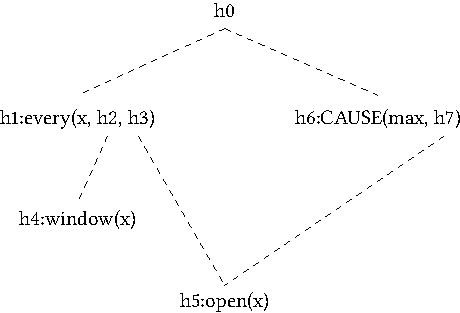
\includegraphics{Figures/max-alle-fenster-oeffnete-mrs-cropped.pdf}
\caption{Dominance graph for \emph{Max alle Fenster öffnete}\label{Abbildung-Max-alle-Fenster-oeffnete}}
\end{figure}%
Each relation in Figure~\ref{Abbildung-Max-alle-Fenster-oeffnete} has a name that one can use to refer to the relation or ``grasp'' it.
These names are referred to as \emph{handle}. The dominance graph states that $h0$ dominates both $h1$ and $h6$ and that
$h2$ dominates $h4$, $h3$ dominates $h5$, and $h7$ dominates $h5$. The exact scopal relations are underspecified: the universal quantifier can have scope over
CAUSE or CAUSE can have scope over the universal quantifier. Figures~\ref{fig-alle-cause} and
\ref{fig-cause-alle} show the variants of the graph with resolved scope.
\begin{figure}
\centering
%% \begin{tabular}{@{}ccc@{}}
%%                                & \mybox[h0]{h0}                & \\[8ex]
%% \mybox[h1]{h1:every(x, \mybox[h2]{h2}, \mybox[h3]{h3})}      &                              & \mybox[h6]{h6:CAUSE(max, \mybox[h7]{h7})}\\[8ex]
%% \mybox[h4]{h4:window(x)}           &         & \\[6ex]
%%                                & \mybox[h5]{h5:open(x)}\\
%% \end{tabular}

%% \begin{tikzpicture}[overlay,remember picture] 
%% \draw(h0.south)--(h1.north); 
%% \draw(h2.south)--(h4.north);
%% \draw(h3.south) .. controls +(0,-1) and +(-1,1)..  (h6.north);
%% \draw(h7.south)--(h5.north);
%% \end{tikzpicture}
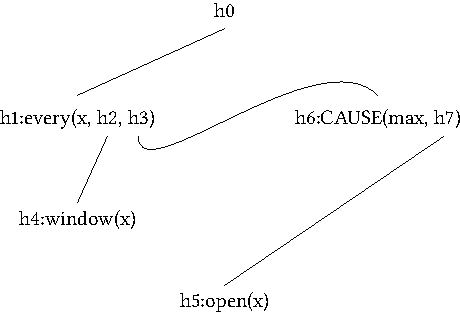
\includegraphics{Figures/solution-mrs-all-cause-open-cropped.pdf}
\caption{Dominance graph for the reading $\forall$ x window(x) $\to$ CAUSE(max,open(x)).\label{fig-alle-cause}}
\end{figure}%
\begin{figure}
\centering
%% \begin{tabular}{@{}ccc@{}}
%%                                & \mybox[h0]{h0}                & \\[8ex]
%% \mybox[h1]{h1:every(x, \mybox[h2]{h2}, \mybox[h3]{h3})}      &                              & \mybox[h6]{h6:CAUSE(max, \mybox[h7]{h7})}\\[8ex]
%% \mybox[h4]{h4:window(x)}           &          & \\[6ex]
%%                                & \mybox[h5]{h5:open(x)}\\
%% \end{tabular}

%% \begin{tikzpicture}[overlay,remember picture] 
%% \draw(h0.south)--(h6.north); 
%% \draw(h7.south) .. controls +(0,-1) and +(-1,1)..  (h1.north);
%% \draw(h2.south)--(h4.north);
%% \draw(h3.south)--(h5.north);
%% \end{tikzpicture}
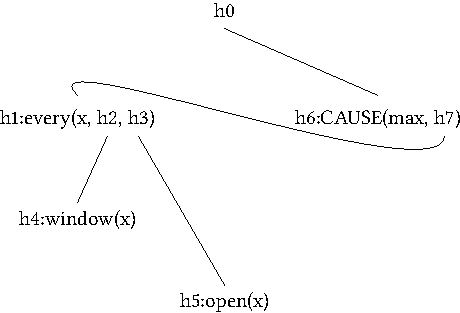
\includegraphics{Figures/solution-mrs-cause-all-open-cropped.pdf}
\caption{Graph for te reading CAUSE(max, $\forall$ x window(x) $\to$ open(x)).\label{fig-cause-alle}}
\end{figure}%
The underspecified graph in Figure~\ref{Abbildung-Max-alle-Fenster-oeffnete} does not say anything
about the relation between $h3$ and $h6$. The only thing it says is that $h3$ somehow has to dominate
$h5$. In Figure~\ref{fig-alle-cause} every ($h3$) dominates CAUSE ($h6$) and CAUSE dominates open
($h5$). So, \relation{every} dominates \relation{open} indirectly. In Figure~\ref{fig-cause-alle}, CAUSE
dominates \relation{every} and \relation{every} dominates \relation{open}. Again the constraints of
Figure~\ref{Abbildung-Max-alle-Fenster-oeffnete} are fulfilled, but $h7$ dominates $h5$ only indirectly.

The fact that the quantifier dominates $h4$ is determined by the lexical entry of the quantifier. The fact that
the quantifier dominates $h5$ does not have to be made explicit in the analysis since the quantifier binds a variable
in the relation belonging to $h5$, namely x. The dominance relation between $h7$ and $h5$ is always determined in the lexicon
since CAUSE and \relation{open}  both belong to the semantic contribution of a single lexical entry.

The exact syntactic theory that one adopts for this analysis is, in the end, not of great importance.
I have chosen HPSG here. As Figure~\vref{Abbildung-Fenster-oeffnete-MRS} shows, the analysis of \emph{alle Fenster öffnet}
contains a simple structure with a verb and an object.
\begin{figure}
%\begin{sideways}
\oneline{%
\begin{forest}
sm edges, for tree={l sep= 4ex}
[V$'$\feattab{
    \subcat \sliste{ NP\ind{y} },\\
    \rels \relliste{ h1:every(x, h2, h3), h4:window(x), h6:CAUSE(y,h7), h5:open(x) },\\
    \hcons \relliste{ h0 \qeq h1, h2 \qeq h4, h0 \qeq h6, h7 \qeq h5 }    }
  [\ibox{2} NP\ind{x}\feattab{
    \rels \relliste{ h1:every(x, h2, h3), h4:window(x) },\\
    \hcons \relliste{ h0 \qeq h1, h2 \qeq h4 } } 
    [Det\feattab{
    \rels \relliste{ h1:every(x, h2, h3) },\\
    \hcons \relliste{ h0 \qeq h1, h2 \qeq h4  } } [alle] ]
    [N\feattab{
    \rels \relliste{ h4:window(x) },\\
    \hcons \relliste{ } } [Fenster] ] ]
  [V\feattab{
                                           \subcat \sliste{ NP\ind{y}, \ibox{2} },\\
                                           \rels \relliste{ h6:CAUSE(y,h7), h5:open(x) },\\
                                           \hcons \relliste{ h0 \qeq h6, h7 \qeq h5 } } [öffnete] ]
]
\end{forest}
}
%\end{sideways}
\caption{\label{Abbildung-Fenster-oeffnete-MRS}MRS analysis of \emph{alle Fenster öffnete}}
\end{figure}%
This structure does not differ from the one that would be assumed for \emph{alle Kinder kennt} `all
children know', involving the semantically simplex verb \emph{kennen} `to know'.
The only difference comes from the meaning of the individual words involved.
As shown in Section~\ref{Abschnitt-HPSG-Semantik}, relations between individual words are passed on upwards.
The same happens with scopal restrictions. These are also represented in lists. \hcons stands for \emph{handle constraints}.
\qeq in h0 \qeq h6 stand for the equality \emph{modulo} quantifier scope.

Egg lists the following readings for the sentence in (\ref{ex-wieder-alle}) -- repeated here as (\mex{1}):
\ea
\label{ex-wieder-alle-zwei}
\gll dass Max wieder alle Fenster öffnete\\
	 that Max again all windows opened\\
\glt `that Max opened all the windows again'
\z
\begin{enumerate}
\item Max opened every window and he had already done that at least once for each window
      (\relation{again}($\forall$(CAUSE(open))); repetitive)
\item Max caused every window to be open and he had done that at least once before 
      (\relation{again}(CAUSE($\forall$(open))); repetitive)
\item At some earlier point in time, all windows were simultaneously open and Max re-established this state
      (CAUSE(\relation{again}($\forall$(open))); restitutive)
\end{enumerate}

\noindent
These readings correspond to the dominance graph in Figure~\vref{Abbildung-Max-wieder-alle-Fenster-oeffnete}.
\begin{figure}
\centering
%%   \begin{tabular}{@{}ccc@{}}
%%   & \mybox[h0]{h0}                       & \\[4ex]
%%     \mybox[h8]{h8:again}\mybox[h9]{(h9)}  \\[4ex]
%%     \mybox[h1]{h1:every(x, \mybox[h2]{h2}, \mybox[h3]{h3})}      &                              & \mybox[h6]{h6:CAUSE(max, \mybox[h7]{h7})}\\[8ex]
%%   \mybox[h4]{h4:window(x)}           &          & \\[6ex]
%%                            & \mybox[h5]{h5:open(x)}\\
%%   \end{tabular}

%% \begin{tikzpicture}[overlay,remember picture,dashed] 
%% \draw(h0.south)--(h8.north); 
%% \draw(h0.south)--(h6.north);
%% \draw(h9.south)--(h1.north);
%% \draw(h2.south)--(h4.north);
%% \draw(h3.south)--(h5.north);
%% \draw(h7.south)--(h5.north);
%% \end{tikzpicture}
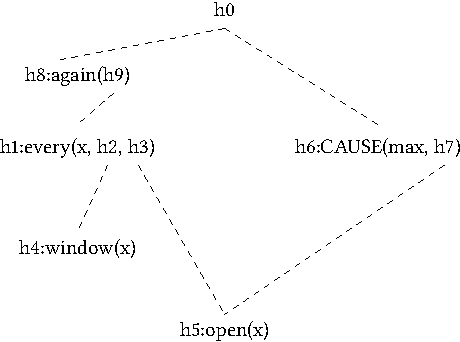
\includegraphics{Figures/mrs-max-wieder-alle-fenster-oeffnete-cropped.pdf}
\caption{Dominance graph for \emph{Max wieder alle Fenster öffnete} `that Max opened all the
  windows again'\label{Abbildung-Max-wieder-alle-Fenster-oeffnete}}
\end{figure}%
Figure~\vref{Abbildung-Max-alle-Fenster-wieder-oeffnete} shows the graph for (\ref{ex-alle-wieder})
-- repeated here as (\mex{1}):\todostefan{Skopus hinzufügen?}
\ea
\label{ex-alle-wieder-zwei}
\gll dass Max alle Fenster wieder öffnete\\
	 that Max all windows again opened\\
\z
\begin{figure}
\centering
%% \begin{tabular}{@{}ccc@{}}
%%                                & \mybox[h0]{h0}                & \\[8ex]
%% \mybox[h1]{h1:every(x, \mybox[h2]{h2}, \mybox[h3]{h3})}      &                              &                               \mybox[h6]{h6:CAUSE(max, \mybox[h7]{h7})}\\[4ex]
%%                                                               \multicolumn{2}{c}{\hspace{3em}\mybox[h8]{h8:again(\mybox[h9]{h9})}}\\[4ex]
%% \mybox[h4]{h4:window(x)}           &          & \\[6ex]
%%                                & \mybox[h5]{h5:open(x)}\\
%% \end{tabular}
%% \begin{tikzpicture}[overlay,remember picture,dashed] 
%% \draw(h0.south)--(h1.north); 
%% \draw(h0.south)--(h6.north);
%% \draw(h2.south)--(h4.north);
%% \draw(h3.south)--(h8.north);
%% \draw(h9.south)--(h5.north);
%% \draw(h7.south)--(h5.north);
%% \end{tikzpicture}
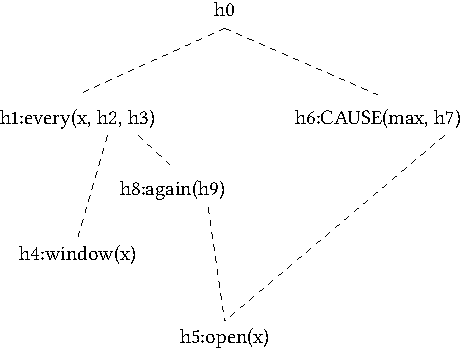
\includegraphics{Figures/mrs-max-alle-fenster-wieder-oeffnete-cropped.pdf}
\caption{Dominance graph for \emph{Max alle Fenster wieder öffnete} `that Max opened all the
  windows again'\label{Abbildung-Max-alle-Fenster-wieder-oeffnete}}
\end{figure}%
To derive these dominance graphs from the ones without \emph{wieder} `again', all one has to do is add the expression h8:again(h9)
and the dominance requirements that demand that $h9$ dominates quantifiers occurring to the right of \emph{wieder} and that it
is dominated by quantifiers to the left of \emph{wieder}.

It is therefore unproblematic to derive the relevant readings for modification by \emph{wieder}
without empty elements for CAUSE and BECOME. The meaning of the word \emph{öffnen} is decomposed in a similar way but the
decomposed meaning is assigned to a single element, the verb. By underspecification of the scopal
relations in the lexicon, the relevant readings can then be derived. 


%% Shravan sagt nee, wahrscheinlich nicht. 24.06.2008
%% Unterspezifikation ist auch psycholinguistisch plausibler als die explizite Ableitung aller Skopus:
%% Es ist unwahrscheinlich, dass Menschen für normale Sätze jeweils Tausende Repräsentationen
%% verwenden, die sich nur in verschiedenen Skopus unterscheiden. Stattdessen lassen sie wahrscheinlich
%% die Bedeutung weitestgehend unterspezifiziert und lösen sie dann bei ausreichendem Kontextwissen
%% weiter auf.

\section{Evidence for empty elements}
\label{Abschnitt-Evidenz-leere-Elemente}

As previously discussed, grammarians agree that both linguists and speakers notice when there is a constituent missing from a
string of words. For cases where it can be shown that analyses with or without traces are indistinguishable empirically,
then one can assume empty elements. Nevertheless, the learnability argument put forward by
Construction Grammarians has some validity: if one assumes that there is no or little innate linguistic knowledge, then it is not possible to motivate empty elements
with data from other languages. This means that just because Basque\il{Basque} shows object agreement\is{agreement!object},
this does not mean that one can assume an empty head for object agreement
(AgrO\is{category!functional!AgrO}) in a grammar of German as
for instance \citet{Stechow96a} and \citet{Meinunger2000a} do. Since there is no object agreement in German, there
would be no way for the child to learn the fact that there is an AgrO head. Knowledge about AgrO
must therefore be innate. Since the assumption of innate linguistic knowledge is controversial (see
Chapter~\ref{chap-innateness}), any theory that uses cross"=linguistic data to motivate the use of empty elements is on shaky ground.

Cross"=linguistic considerations can only be drawn upon if there are no empirical differences between multiple alternative
analyses compatible and motivated by the language under consideration. In this case, one should follow Occam's Razor and choose the analysis which is compatible with analyses of
other languages (see \citealp{MuellerCoreGram} and Chapter~\ref{sec-develop-theories-coregram}).
\is{empty element|)}


\section{Transformations, lexical rules, and empty elements}
\label{Abschnitt-leere-Elemente-LRs-Transformations}

In\is{empty element|(}\is{lexical rule|(}\is{transformation|(} the discussion of the passive\is{passive} in the framework of TAG, it became clear that lexical rules
correspond to particular transformations, namely those which have some relation to a lexical item (lexically governed transformations, \citealp{Dowty78a}; 
for the discussion of transformations and lexical rules, see \citew{Bresnan78a} and \citew{BK82a}). In the respective variants of TAG\indextag, lexical rules establish a relation
between a lexical item for an active tree with a lexical item of a passive tree. Both the active and passive tree can be extended by adjunction.

In theories such as Categorial Grammar\indexcg, the situation is similar: since the direction in which a functor expects to find its argument is fixed
for languages such as English, the lexical item stands for an entire tree. Only the attachment of
adjuncts is not yet specified in lexical items. The positions in the
tree where the adjuncts can occur depend on the properties of the adjuncts. In Section~\ref{Abschnitt-CG-lokale-Umstellung},
we have seen suggestions for treatments of languages with free constituent order. If the direction of combination is not fixed in the lexicon, then the lexical item
can occur in a number of trees. If we compare lexical rules that can be applied to this kind of lexical items with transformations, we see that lexical rules create relations
between different sets of trees.

In \hpsg analyses\indexhpsg, this works in a similar way: lexical rules relate lexical items with differing valence properties to each other. In HPSG grammars of English\il{English},
there is normally a schema that licenses a VP containing the verb and all its complements as well as a schema that connects the subject to the VP 
\citep[\page 39]{ps2}. In the lexical items for finite verbs, it is already determined what the tree will look like in the end. As in Categorial Grammar, adjuncts in HPSG can
be combined with various intermediate projections. Depending on the dominance schemata used in a particular grammar, the lexical item will determine the constituent structure
in which it can occur or allow for multiple structures. In the grammar of German proposed in Chapter~\ref{Kapitel-HPSG}, it is possible to analyze six different sequences with a lexical
item for a ditransitive verb, that is, the lexical item can -- putting adjuncts aside -- occur in six different structures with verb"=final order. Two sequences can be analyzed
with the passive lexical item, which only has two arguments.
As in Categorial Grammar, sets of licensed structures are related to other sets of licensed structures. In HPSG theorizing and also in Construction Grammar, there have been
attempts to replace lexical rules with other mechanisms since their ``status is dubious and their interaction with other analyses is controversial''
\citep*[\page 19]{BMS2001a}. \citet{BMS2001a} propose an analysis for extraction
that, rather than connecting lexical items with differing valence lists, establishes a relation between a subset of a particular list in a lexical item and another
list in the same lexical item. The results of the two alternative analyses are shown in (\mex{1})
and (\mex{2}), respectively:
\eal
\ex \ms{ subcat & \sliste{ NP[\type{nom}], NP[\type{acc}] }\\
         slash  & \eliste\\
       }
\ex \ms{ subcat & \sliste{ NP[\type{nom}] }\\
         slash  & \sliste{ NP[\type{acc}] }\\
       }
\zl
\addlines
In (\mex{0}), (\mex{0}a) is the basic entry and (\mex{0}b) is related to (\mex{0}a) via a lexical
rule. The alternative analysis would only involve specifying the appropriate value
of the \textsc{arg-st} feature\footnote{
\argst stands for \emph{Argument Structure}. The value of \argst is a list containing all the arguments
of a head. For more on \argst, see Section~\ref{Abschnitt-Arg-St}.
}\isfeat{arg-st} and the \subcat and \slashv is then derived from the \argstv using the relevant constraints.
(\mex{1}) shows two of the licensed lexical items.
\eal
\ex \ms{ arg-st & \sliste{ NP[\type{nom}], NP[\type{acc}] }\\
         subcat & \sliste{ NP[\type{nom}], NP[\type{acc}] }\\
         slash  & \eliste\\
       }
\ex \ms{ arg-st & \sliste{ NP[\type{nom}], NP[\type{acc}] }\\
         subcat & \sliste{ NP[\type{nom}] }\\
         slash  & \sliste{ NP[\type{acc}] }\\
       }
\zl
If we want to eliminate lexical rules entirely in this way, then we would require an additional feature for each change.\footnote{
Alternatively, one could assume a very complex relation that connects \argst and \subcat. But this would then have to deliver
the result of an interaction of a number of phenomena and the interaction of these phenomena would not be captured in a transparent way.%
} Since there are many interacting valence"=changing processes, things only work out with the stipulation of a large number of auxiliary
features. The consequences of assuming such analyses have been discussed in detail in
\citew[Section~7.5.2.2]{MuellerLehrbuch1}. The problems that arise are parallel for
inheritance"=based approaches for argument structure"=changing processes: they also require
auxiliary features since it is not possible to model embedding and multiple changes of valence information with inheritance. See Section~\ref{Abschnitt-Passiv-CxG}.

Furthermore, the claim that the status of lexical rules is dubious must be rejected: there are worked"=out formalizations of lexical rules \citep{Meurers2001a,CB92a,LC99a}
and their interaction with other analyses is not controversial. Most HPSG implementations make use of lexical rules and the interaction of a number of rules and
constraints can be easily verified by experiments with implemented fragments.

\citet{Jackendoff75a} presents two possible conceptions of lexical rules: in one variant, the lexicon contains all words in a given language and there
are just redundancy rules saying something about how certain properties of lexical entries behave with regard to properties of other lexical entries. For example,  \stem{les} `read-' and \emph{lesbar}
`readable' would both have equal status in the lexicon. In the other way of thinking of lexical
rules, there are a few basic lexical entries and the others are derived
from these using lexical rules. The stem  \stem{les} `read-' would be the basic entry and \emph{lesbar} would be derived from it.
In HPSG, the second of the two variants is more often assumed. This is equivalent to the assumption of unary rules. In Figure~\ref{Abbildung-Verbstellung-HPSG} on
page~\pageref{Abbildung-Verbstellung-HPSG}, this has been shown accordingly: the verb \emph{kennt}
`knows' is mapped by a lexical rule to a verb that selects the projection of an
empty verbal head. With this conception of lexical rules, it is possible to remove lexical rules from the grammar by assuming binary"=branching structures with an
empty head rather than unary rules. For example, in HPSG analyses of resultative constructions\is{resultative construction}\is{construction!resultative|(}
such as (\mex{1}), lexical rules have been proposed (\citealp{Verspoor97a}; \citealp{Wechsler97a}; \citealp{WN2001a}; \citealp[Chapter~5]{Mueller2002b}).
\ea
\gll [dass] Peter den Teich leer fischt\\
	 \spacebr{}that Peter the pond empty fishes\\
\glt `that Peter fishes the pond empty'
\z
In my own analysis, a lexical rule connects a verb used intransitively to a verb that selects an accusative object and a predicate.
Figure~\vref{Abbildung-Resultativ-LR} shows the corresponding tree.
\begin{figure}
\centering
\begin{forest}
sm edges
[V{[\subcat \eliste]}
	[NP{[\type{nom}]}
		[Peter;Peter]]
	[V{[\subcat \sliste{ NP[\type{nom}] }]}
		[NP{[\type{acc}]}
			[den Teich;the pond, roof]]
		[V{[\subcat \sliste{ NP[\type{nom}], NP[\type{acc}] } ]}
			[Adj
				[leer;empty]]
			[V{[\subcat \sliste{ NP[\type{nom}], NP[\type{acc}], Adj } ]}
				[V{[\subcat \sliste{ NP[\type{nom}]} ]}
					[fischt;fishes]]]]]]
\end{forest}
\caption{\label{Abbildung-Resultativ-LR}Analysis of the resultative construction with a lexical rule}
\end{figure}%
If we consider what (\mex{0}) means, then we notice that the fishing act causes the pond to become empty.
This causation is not contained in any of the basic lexical items for the words in (\mex{0}).
In order for this information to be present in the semantic representation of the entire expression, it has
to be added by means of a lexical rule. The lexical rule says: if a verb is used with an additional predicate and accusative
object, then the entire construction has a causative meaning.

Figure~\vref{Abbildung-Resultativ-leer} shows how a lexical rule can be replaced by an empty head.
\begin{figure}
\centering
\begin{sideways}
%\scalebox{0.9}{%
\begin{forest}
sm edges
[V{[\subcat \eliste]}
	[{NP[\type{nom}]}
		[Peter;Peter]]
	[{V[\subcat \sliste{ NP[\type{nom}] }]}
		[{NP[\type{acc}]}
			[den Teich;the pond,roof]]
		[{V[\subcat \sliste{ NP{[\type{nom}]}, NP{[\type{acc}]} }]}
			[Adj
				[leer;empty]]
			[{[\subcat \sliste{ NP{[\type{nom}]}, NP{[\type{acc}]}, Adj }]}
				[{V[\subcat \sliste{ NP{[\type{nom}]} }]}
					[fischt;fishes]]
				[{V[\subcat \sliste{ NP{[\type{nom}]}, NP{[\type{acc}]}, Adj, V{[\subcat \sliste{ NP{[\type{nom}]} }]} }]}
					[\trace]]]]]]
\end{forest}
%}
\end{sideways}
\caption{\label{Abbildung-Resultativ-leer}Analysis of the resultative construction with an empty head}
\end{figure}%
The empty head requires the intransitive verb and additionally an adjective, an accusative object and a subject.
The subject of \emph{fischt} `fishes' must of course be identical to the subject that is selected by the combination
of \emph{fischt} and the empty head. This is not shown in the figure.
It is possible, however, to establish this identity (see \citealp{HN94a}). The causative semantics is contributed by
the empty head in this analysis. The trick that is being implemented here is exactly what was done in Section~\ref{Abschnitt-Eleminierung-leerer-Elemente},
just in the opposite direction: in the previous section, binary"=branching structures with an empty daughter were replaced by unary"=branching structures.
In this section, we have replaced unary"=branching structures with binary"=branching structures with an empty daughter.\footnote{
	Here, we are discussing lexical rules, but this transformation trick can also be applied to
        other unary rules. Semanticists often use such rules for type shifting\is{type raising}. For
        example, a rule that turns a referential NP such as \emph{a trickster} in (i.a) into a
        predicative one (i.b) \citep{Partee87a-u}.
\eal
\ex A trickster laughs.
\ex He is a trickster.
\zl
These changes can be achieved by a unary rule that is applied to an NP or with a special empty head that takes an NP as its argument. In current Minimalist\indexmp approaches,
empty heads are used \citep[\page 370]{Ramchand2005a}, in Categorial Grammar\indexcg and HPSG\indexhpsg unary"=branching rules are more common (\citealp[\page
    91--92]{Flickinger2008a}; \citealp{MuellerPredication,MuellerCopula}).
}\is{empty element|)}\is{lexical rule|)}\is{transformation|)}\is{construction!resultative|)}

\largerpage
We have therefore seen that certain transformations can be replaced by lexical rules and also that
lexical rules can be replaced by empty heads. 
The following chapter
%will deal with the question of whether meaning is contributed by lexical heads or rather holistically by phrasal configurations.
deals with the question of whether phenomena like extraction, scrambling, and passive should be
described with the same tool as in GB/Minimalism or with different tools as in LFG and HPSG.



%      <!-- Local IspellDict: en_US-w_accents -->
